\documentclass[
    9pt,            % 8-20pt possible
    % twocolumn,      % switch, use twocolumn layout
    commun,        % select between  ``techreport'', ``report'', ``article'', ``commun'', ``persp'' and ``review''
    % lineno,         % switch, adds line numbering
    % tocfig,         % switch, use a TOC figure at the top (place in ./figs)
    % SI,             % switch to Supplemental Information format, not compatible with twocolumn
    affiltop,       % switch, put affiliations under authors (instead of footnote)
    % nofootprint,    % do not add "Preprint" in footer
    % nofootdate,     % do not add date in footer
    % debug,          % switch, add debugging boxes
    % draft,          % for quick compilations (no figures, references etc)
]{art}


% Title
\newcommand{\pubtitle}{
    {Anoma: a unified architecture for full-stack decentralised applications}}

\newcommand{\pubauthA}{Christopher Goes}
\newcommand{\pubaffilA}{a}
% \newcommand{\orcidA}{0000-0001-5477-1503}
\newcommand{\authemailA}{sherlock@heliax.dev}
% \newcommand{\eqcontribA}{}

\newcommand{\pubauthB}{Awa Sun Yin}
\newcommand{\pubaffilB}{a}
% \newcommand{\orcidB}{0000-0001-0000-0000}
\newcommand{\authemailB}{poison@heliax.dev}
% \newcommand{\eqcontribB}{}

\newcommand{\pubauthC}{Adrian Brink}
\newcommand{\pubaffilC}{a}
% \newcommand{\orcidC}{0000-0001-5477-1503}
% \newcommand{\authemailC}{mail@someinstitute.com}

% Institutions/Affiliations
\newcommand{\pubaddrA}{Heliax AG}

% Corresponding author mail
\newcommand{\pubemail}{\authemailA}

\newcommand{\pubabstract}{%
Programmable settlement architectures do not enable counterparty discovery
and solving, both of which are necessary to build the majority of
interactive multi-party applications. The architectural constraints of
programmable settlement result in contemporary application protocols that
have at least one Web2 component, which becomes the centralisation point.
We present Anoma, a unified architecture for full-stack decentralised
applications. Anoma is designed following the principles of
intent-centricity and homogeneous architecture / heterogeneous security,
together constituting a declarative paradigm for building decentralised
applications. In this paper, we first outline the Anoma architecture,
provide an intuition for the design rationale, and describe how Anoma
disentangles the choices of protocol and security. We then define the Anoma
application programming model and enumerate several existing and novel
decentralised applications that can be built using the novel primitives.
Finally, we outline the current components used to instantiate Anoma and
list future research directions.
}

% Description of the SI file, placed as a footnote
% \newcommand{\pubSI}{Electronic Supplementary Information (ESI) available:
% one PDF file with all referenced supporting information.}

% Any keywords to be displayed under the abstract
\keywords{ 
Anoma \sep 
Intent-Centricity and Homogeneous Architecture \sep 
Full-Stack Decentralised Applications \sep
Counterparty Discovery \sep 
Programmable Settlement Architectures \sep
}

% Supplementary space between title/abstract and text, if needed
% \newcommand{\pubVadj}{0pt}

% ! DO NOT REMOVE OR MODIFY !
% Do not modify this file!

\title{\pubtitle}

\newcommand{\dg}{\textsuperscript{\textbf{\dag\textnormal{,}}}}

\ifdef{\pubauthA}{\author[\pubaffilA]{\pubauthA\ifdef{\orcidA}{~\protect\orcid{\orcidA}}{}\ifdef{\eqcontribA}{\dg}{}}}{}
\ifdef{\pubauthB}{\author[\pubaffilB]{\pubauthB\ifdef{\orcidB}{~\protect\orcid{\orcidB}}{}\ifdef{\eqcontribB}{\dg}{}}}{}
\ifdef{\pubauthC}{\author[\pubaffilC]{\pubauthC\ifdef{\orcidC}{~\protect\orcid{\orcidC}}{}\ifdef{\eqcontribC}{\dg}{}}}{}
\ifdef{\pubauthD}{\author[\pubaffilD]{\pubauthD\ifdef{\orcidD}{~\protect\orcid{\orcidD}}{}\ifdef{\eqcontribD}{\dg}{}}}{}
\ifdef{\pubauthE}{\author[\pubaffilE]{\pubauthE\ifdef{\orcidE}{~\protect\orcid{\orcidE}}{}\ifdef{\eqcontribE}{\dg}{}}}{}
\ifdef{\pubauthF}{\author[\pubaffilF]{\pubauthF\ifdef{\orcidF}{~\protect\orcid{\orcidF}}{}\ifdef{\eqcontribF}{\dg}{}}}{}
\ifdef{\pubauthG}{\author[\pubaffilG]{\pubauthG\ifdef{\orcidG}{~\protect\orcid{\orcidG}}{}\ifdef{\eqcontribG}{\dg}{}}}{}
\ifdef{\pubauthH}{\author[\pubaffilH]{\pubauthH\ifdef{\orcidH}{~\protect\orcid{\orcidH}}{}\ifdef{\eqcontribH}{\dg}{}}}{}
\ifdef{\pubauthI}{\author[\pubaffilI]{\pubauthI\ifdef{\orcidI}{~\protect\orcid{\orcidI}}{}\ifdef{\eqcontribI}{\dg}{}}}{}
\ifdef{\pubauthJ}{\author[\pubaffilJ]{\pubauthJ\ifdef{\orcidJ}{~\protect\orcid{\orcidJ}}{}\ifdef{\eqcontribJ}{\dg}{}}}{}
\ifdef{\pubauthK}{\author[\pubaffilK]{\pubauthK\ifdef{\orcidK}{~\protect\orcid{\orcidK}}{}\ifdef{\eqcontribK}{\dg}{}}}{}

\ifdef{\eqcontribA}{\equalcontrib{}}{}
\ifdef{\eqcontribB}{\equalcontrib{}}{}
\ifdef{\eqcontribC}{\equalcontrib{}}{}
\ifdef{\eqcontribD}{\equalcontrib{}}{}
\ifdef{\eqcontribE}{\equalcontrib{}}{}
\ifdef{\eqcontribF}{\equalcontrib{}}{}
\ifdef{\eqcontribG}{\equalcontrib{}}{}
\ifdef{\eqcontribH}{\equalcontrib{}}{}
\ifdef{\eqcontribI}{\equalcontrib{}}{}
\ifdef{\eqcontribJ}{\equalcontrib{}}{}
\ifdef{\eqcontribK}{\equalcontrib{}}{}

\ifdef{\pubaddrA}{\affil[a]{\pubaddrA}}{}
\ifdef{\pubaddrB}{\affil[b]{\pubaddrB}}{}
\ifdef{\pubaddrC}{\affil[c]{\pubaddrC}}{}
\ifdef{\pubaddrD}{\affil[d]{\pubaddrD}}{}
\ifdef{\pubaddrE}{\affil[e]{\pubaddrE}}{}
\ifdef{\pubaddrF}{\affil[f]{\pubaddrF}}{}
\ifdef{\pubaddrG}{\affil[g]{\pubaddrG}}{}
\ifdef{\pubaddrH}{\affil[h]{\pubaddrH}}{}

\contact{\pubemail}

%% Abstract
%% --------

\begin{abstract}
    \pubabstract{}
\end{abstract}

%% Keywords
%% --------

\ifdef{\pubkeywords}{\keywords{\pubkeywords}}{}

%% Adjusting vertical space
%% ------------------------

\ifdef{\pubVadj}{\verticaladjustment{\pubVadj}}{}

% The preprint DOI to be used as an link in the paper
\pubdoi{10.5281/zenodo.8262747}
\history{(Received August 21, 2022; Published: August 21, 2022; Version: \today)}
% MACROS
\newcommand{\N}{\mathbb{N}}

\newcommand{\JuvixCore}{\ensuremath{\mathsf{JuvixCore}}}
\newcommand{\Geb}{\ensuremath{\mathsf{Geb}\,}}
\newcommand{\Juvix}{\ensuremath{\mathsf{Juvix}}}
\newcommand{\VampIR}{\ensuremath{\mathsf{VampIR}}}
\newcommand{\LambdaIR}{\ensuremath{\mathsf{Lambda}}}


\begin{document}

\maketitle

\tableofcontents

\section{Background and motivations}\label{background-and-motivations}

The release of the Bitcoin protocol in 2008 marked the beginning of
\emph{scriptable settlement}, a category of distributed ledger
architectures that is suitable for cryptocurrencies with discrete
properties and monetary policies. Although it is not Turing-complete,
Bitcoin Script~\cite{bitcoinscript} is able to support applications beyond
currencies, such as Namecoin and Colored Coins. As discussed in the
Ethereum Whitepaper~\cite{ethereumwhitepaper}, while applications built on
scriptable settlement are functional, this architecture requires too many
trade-offs that resulted in constrained properties and usability.

The introduction of the Ethereum protocol in 2014 set the precedent for
\emph{programmable settlement}, a new category of architectures for
constructing decentralised applications that leverage Turing-complete
virtual machine execution, which adds substantially more expressivity to
the settlement layer. Programmable settlement paved the way for improved
versions of applications that scriptable settlement is not able to support,
such as fungible tokens (ERC20) or Ethereum Name Service (ENS), which are
today well-established versions of the Colored Coin and Namecoin ideas,
respectively -- in addition to many other desirable applications, such as
non-fungible tokens (NFTs), Decentralised Autonomous Organisations (DAOs),
or the recently introduced Soulbound Tokens
(SBTs)~\cite{weyl2022decentralized}.

Proposed and deployed blockchain protocols since Ethereum's
release have brought significant improvements to specific architectural
components, for instance: consensus mechanisms
(Tendermint~\cite{buchman2018latest}, Avalanche~\cite{rocket2018snowflake}),
Sybil-resistance mechanisms (proof-of-stake, proof-of-storage), scaling
solutions (sharding, rollups), and cryptographic schemes (zero-knowledge
proofs) -- but these improvements to constituent primitives do not change
the basic architecture of programmable settlement.

While programmable settlement is sufficient for certain applications,
many contemporary applications have further requirements. Settlement
suffices when the involved parties have already decided what and with
whom to settle, but contemporary applications often also require
infrastructure for helping potential counterparties discover each other
and decide with whom and on what to settle. As a workaround, existing
applications have usually adopted an architecture that relies on one or
many permissioned or centralised components (such as provers, solvers,
or sequencers), usually implemented as Web2 services, in their stack.

Examples include decentralised exchanges for fungible assets (0x,
CoWSwap, Uniswap), for non-fungible assets (Wyvern, LooksRare, OpenSea),
novel voting/funding mechanisms (quadratic voting/funding, Gitcoin), and
rollups (Optimism, Arbitrum, Starknet, zkSync) -- their architectures
involve at least one centralised component that often results in a loss
of permissionlessness, fault-tolerance, censorship-resistance, or
privacy.

One emerging approach for applications seeking to avoid centralisation
points in their architecture is to deploy an application-specific
sovereign chain to replace a specific component in the stack. Even
though this approach can solve the immediate centralisation problem, it
comes with substantial trade-offs, such as the loss of network effects
(application composability and software re-use) or the addition of
disproportionate complexity to developers and users, who need to reason
about multi-layered security, privacy, and latency domains.

In this paper we present Anoma. Anoma is a unified architecture for
full-stack decentralised applications -- characterised by its
intent-centricity, decentralised counterparty discovery and computational
outsourcing of NP search problems to solvers which compute valid state
transitions. With this architecture, contemporary applications can be built
without compromising permissionlessness, fault-tolerance,
censorship-resistance, or privacy.

Anoma's architecture also exposes novel primitives, such as
composable privacy, which enables applications to handle transparent,
shielded, and private state and operations; and multi-chain atomic
settlement, which allows users and applications with different security
preferences to obtain atomicity. These and other novel primitives pave the
way for the development of applications that cannot be built with existing
architectures, several of which we enumerate in \textbf{Section 5:
Applications}.

\section{Architectural design philosophy}\label{architectural-design-philosophy}

Anoma's architecture is driven by two design principles:
first, intent-centricity; second, a homogeneous protocol architecture
with a heterogeneous security model. Beyond these two design principles,
all other architectural choices are a matter of modularisation and
runtime configuration parameters.

\subsection{Intent-centricity}\label{intent-centricity}

An \emph{intent} is an expression of what a user wants to achieve
whenever they interact with a protocol, for instance "transfer X from A
to B" or "trade X for Y". Practically, an intent is an off-chain signed
message that encodes which state transitions a user wants to achieve.
Unlike transactions, intents are partial, so one can think of intents as
parts of transactions that require other direct or indirect parts as
complements in order to form a final balanced transaction which
satisfies all users' constraints.

Existing protocols are designed with \emph{transactions} as their most
fundamental unit. Anoma takes a radically different approach: the
architecture of Anoma is centred around programmatic \emph{intents}.

An intent-centric architecture is necessary to enable counterparty
discovery, which is crucial for compelling applications, since they
require multiparty coordination and to enable full-stack decentralised
applications. Anoma vertically integrates counterparty discovery,
solving, and settlement, and is able to interpret and process intents
natively and generically. Contemporary applications, as described
earlier, require both counterparty discovery, solving, and settlement.
Intents are the point at which users interact with such applications,
and an intent-centric design captures the requirements of applications
which need these two processes to work in tandem and satisfy
censorship-resistance, privacy, and fault-tolerance properties.

Intent-centric design also constitutes a \emph{declarative paradigm} for
building applications, since Anoma is designed to settle intents
\emph{as defined} by the users -- an intent is either settled as
defined, or not settled at all. This declarative model gives users a
significantly higher degree of control, \emph{without} requiring them to
understand the underlying protocol primitives and execution flows, which
is crucial in order for decentralised applications to reach mass
adoption. This paradigm presents a radically different approach as
compared to existing \emph{transaction-centric} architectures that
default to an \emph{imperative model} for applications. In the latter,
users are required to understand the full execution trace to benefit
from security and privacy guarantees, because instead of authorising a
specific state change, they authorise specific execution paths. In
practice, this is so difficult that users commonly interact with
applications without understanding the risks.

For application developers, Anoma's intent-centric
architecture enables them to build \emph{safer by construction
applications} by leveraging the combination of intents and \emph{validity
predicates}. Validity predicates are an architecture for smart contracts
which separate out cleanly the task of computing state transitions and the
task of verifying correctness of state transitions, as compared to
message-passing VM execution models (pervasive in current programmable
settlement architectures) which interleaves computation and verification.
Validity predicates allow application developers to reason about the
invariants which they would like their application to satisfy without
worrying about how other applications interact with it, since the validity
predicate of their application expresses these invariants directly.

\subsection{Homogeneous architecture, heterogeneous
security}\label{homogeneous-architecture-heterogeneous-security}

The Anoma protocol, just like the TCP/IP protocol stack, follows the
principle of homogeneous architecture and heterogeneous security. In
TCP/IP, the various layers of the internet protocol are standardised, but
the choice of whom to connect to and what data to entrust them with is left
to the user, and different users can make different choices while using the
same protocol stack. In Anoma, the various layers of counterparty
discovery, solving, and settlement are similarly standardised, but the
choice of what security domains to trust and what data to send to whom are
left to the user, and different users can make different choices while
using the same protocol stack.

In this framework, protocols can be analysed along two dimensions:
architecture and security.

\begin{itemize}
\item
  \textbf{Architecture}: the abstractions and relations constituting the
  structure of a system. An architecture is syntactical, possessed of
  properties and syntaxes but with no particular semantics in relation to
  the exterior world. Convergence on a singular architecture saves time and
  verification costs without constraining users to particular choices.
\item
  \textbf{Security}: the choice of whom and how to trust in the operation
  of a distributed system. Security is a decision inseparable from the
  particular semantics of a specific context of use. While security can be
  economically abstracted to a certain degree by limiting the information
  available to and consequent choice-making capabilities of system
  operators, operators will always have choices of: how and from whom to
  accept messages; when to elect to include them in blocks or other
  aggregations over which they vote; and when to cease voting or otherwise
  alter normal operational procedures in response to exceptional
  circumstances. Whom to trust with these responsibilities depends on what
  the state in the database \emph{represents} in the real world, and
  alignment with the interests of users of the database requires mutual
  interests beyond the purely economic ones.
\end{itemize}

\subsubsection{Analysis of platforms}\label{analysis-of-platforms}

Consider distributed ledger platforms, from the perspective of applications
running on top of them, along these two dimensions: protocol architecture
and security model, and whether they
are~\emph{homogeneous}~or~\emph{heterogeneous}~for different applications
running on the same platform.

Protocol architecture refers to the state layout, virtual machine, language
support, sharding mechanisms, cross-contract messaging model, etc. An
architecture determines what is required to write an application for a
platform, and applications are specific to a particular architecture.

\begin{itemize}

\item
  Platforms with a~\emph{homogeneous}~architecture require that all
  applications are written in a certain format (e.g. EVM bytecode or
  WASM).
\item
  Platforms with a~\emph{heterogeneous}~architecture allow applications
  to be written in different formats, perhaps with some agreement at the
  edges, such as cross-chain communication protocols.
\end{itemize}

Security model refers both to security~\emph{in theory}, such as fault
tolerance properties of the consensus, fork detection and handling; and
security~\emph{in practice}, i.e. which miners or validators operate the
deployed instances of these architectures.

\begin{itemize}

\item
  Platforms with a~\emph{homogeneous}~security model have the same
  security for all applications.
\item
  Platforms with a~\emph{heterogeneous}~security model have different
  security characteristics for different applications.
\end{itemize}

For illustration, \Cref{tab:platforms} situates several platforms on these
two axes:

\begin{table}[H] 
  \label{tab:platforms}
\centering
\begin{tabular}{lll}
\toprule 
\textbf{Platform} & \textbf{Architecture} & \textbf{Security Model}\\
\midrule 
Bitcoin & Homogeneous & Homogeneous\\
Ethereum & Homogeneous & Homogeneous\\
Ethereum 2.0 & Homogeneous & Homogeneous\\
Polkadot & Heterogeneous & Homogeneous\\
Near & Homogeneous & Homogeneous \\
Cosmos & Heterogeneous & Heterogeneous\\
Multichain & Heterogeneous & Heterogeneous\\
Anoma & Homogeneous & Heterogeneous\\
\bottomrule
\end{tabular} 
\caption{An analysis of platforms based on their architecture and security model}
\end{table}

  
% \begin\{table\}{[}h} \centering
% \begin\{tabularx\}\{\linewidth\}{[}t}\{lll\}
% \toprule \textbf\{Platform\} \&
% \textbf\{Architecture\} \& \textbf\{Security
% Model\\/\midrule Bitcoin \& Homogeneous \&
% Homogeneous\/Ethereum \& Homogeneous \& Homogeneous\/Ethereum 2.0 \& Homogeneous \& Homogeneous\/Polkadot \& Heterogeneous \& Homogeneous\/Near \& Homogeneous \& Homogeneous \textbackslash{}
% Cosmos \& Heterogeneous \& Heterogeneous\/Multichain \&
% Heterogeneous \& Heterogeneous\/Anoma \& Homogeneous \&
% Heterogeneous\/\bottomrule
% \end\{tabularx\} \caption\{An analysis of
% platforms based on their architecture and security model\}
% \end\{table\}

As the table suggests, these dimensions are generally quite correlated:
homogeneous architectures come with homogeneous security models, and
heterogeneous architectures come with heterogeneous security models. It
is easier to design a system where they are correlated. If everything is
homogeneous, protocols can be fit together neatly, and functionalities
including cross-contract communication are easy; whereas if everything
is heterogeneous, protocols just agree on the edges of interaction, for
instance via the Inter-Blockchain Communication protocol
(IBC)~\cite{goes2020interblockchain}, and handling the complexity of
security is up to the users and application developers.

\subsubsection{Why decouple these
dimensions?}\label{why-decouple-these-dimensions}

Anoma's fractal instance architecture is designed to
decouple these dimensions and build a platform which is
architecturally~\emph{homogeneous} and with
a~\emph{heterogeneous}~security model. This is more complicated, but it
separates out the question of what the best~\emph{protocol architecture}
is, where there may be a "benevolent monopoly" (à la Git or TCP/IP),
from the question of what is the best~\emph{security model}, where there
is almost certainly not.

Applications written for fractal instances can standardise on the
architecture Anoma offers, which is sufficiently well-defined to allow
for complex interoperability, automatic scaling, etc., without agreeing
on any single security model. Furthermore, in some cases, this
flexibility of choice can be extended all the way to users of the
applications, who can choose independently.

User interfaces for Anoma instances can support the same applications
deployed with different security models, and communicate that latter
difference to users in a way which allows them to choose their trust
assumptions while retaining the network effects of using the same
protocol.

Noteworthily, Anoma's architecture is not homogeneous
like a straitjacket, as it supports multiple deployment models. The
components in the protocol are layered so that fractal instances can
pick and choose which parts they participate in, even if it involves
leveraging Anoma for specific functionalities, such as decentralised
counterparty discovery and solving, whilst anchoring the final
settlement on another platform, such as Ethereum. Nonetheless, a unified
and vertically integrated architecture allows developers and users to
benefit from standardisation.

\section{Architectural topology}\label{architectural-topology}

Anoma's architectural topology consists of a set of
logical abstractions delineated by their role in dataflow, independent
of particular forms of representation, deployment models, choices of
cryptographic implementation, etc, \textbf{Figure 1} provides an
overview of the architectural topology. Particular instantiations carry
different concrete performance and security implications and should be
chosen according to requirements of the specific deployment in question.
We offer a sketch of our choices for different deployments in
\textbf{Section 5: Applications}.

\begin{figure*}
  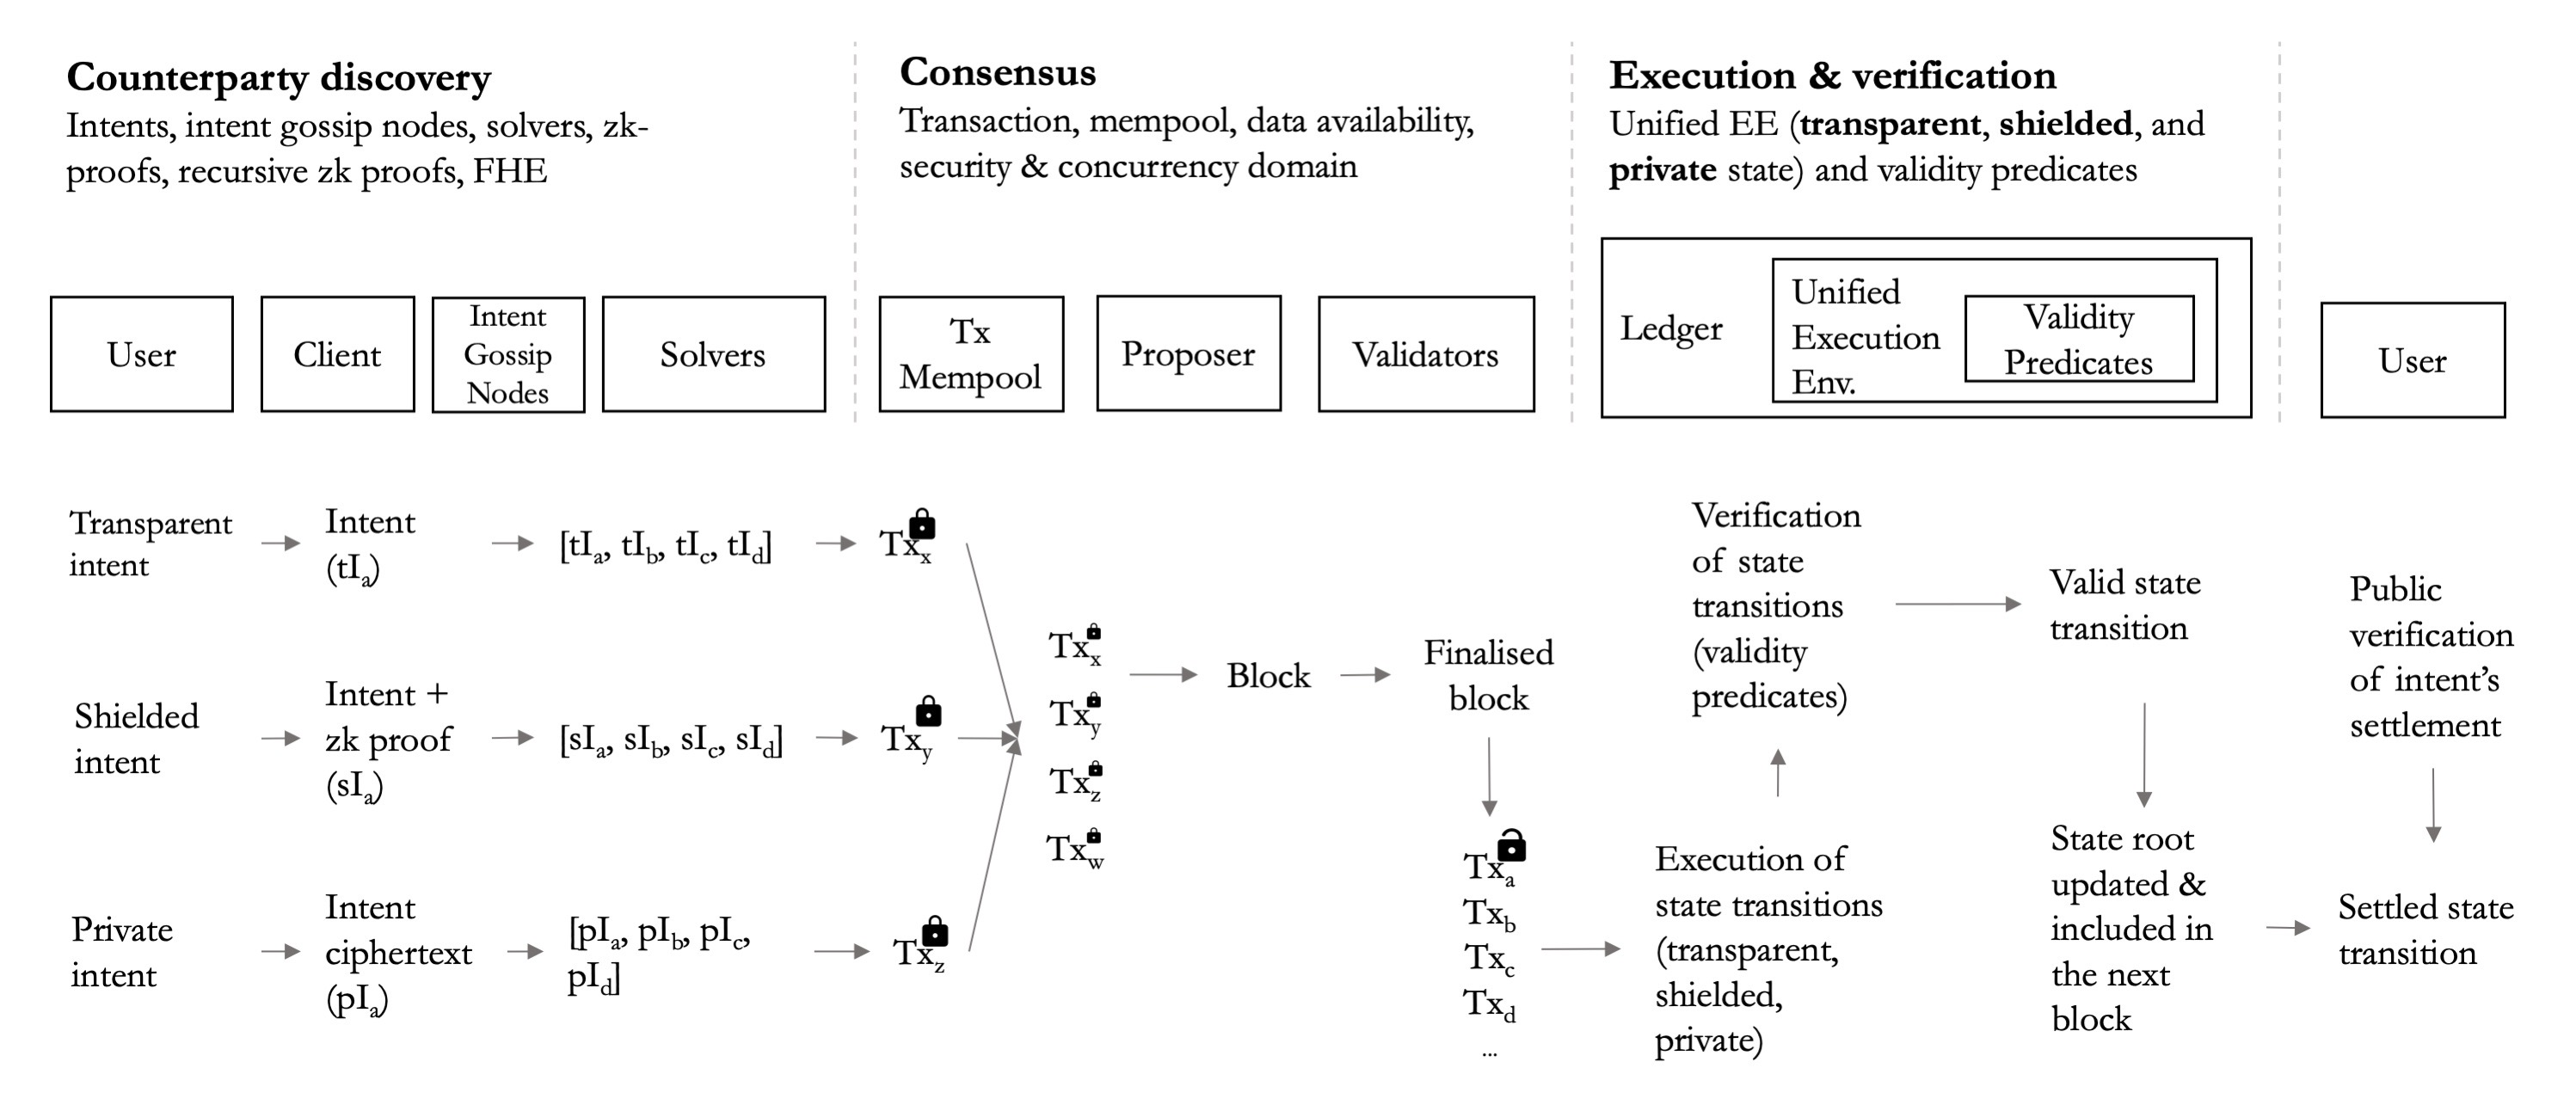
\includegraphics[width=\textwidth,keepaspectratio]{figs/intents-lifecycle.jpeg}
  \caption{The lifecycle of a transparent, shielded, and private intent in the Anoma architecture}
\end{figure*}
  

\subsection{Nodes and network layer}\label{nodes-and-network-layer}

The architectural topology of Anoma operates on a substrate of networked
Turing machines, which we refer to as \emph{nodes}. Nodes may take on
different operational \emph{roles}, such as gossiping intents, searching
for solutions, and voting in consensus. Although different roles will
have different hardware requirements, nodes are a single class and
runtime configuration settings determine which roles a node performs.

All nodes compute deterministically, with the ability to generate local
randomness (which may be used, for example, as secret values in
cryptography) and have read and write access to local storage. The set
of nodes is unbounded and dynamic with nodes entering and exiting at any
times. Nodes are partially connected on an open network, where different
roles require different connections. The network layer is assumed to be
unreliable (messages may be arbitrarily dropped, duplicated, or
reordered) and untrustworthy (unencrypted data is not secret). Specific
roles may have more stringent network assumptions such as partial
synchrony.

\subsection{Intents}\label{intents}

An \emph{intent} is a signed message that describes a partial state
transitions. Semantically, intents contain information about state
preferences, such as that Alice wishes to swap X for Y, or any X with
property T for any Y with property U, or Z for some asset A, but only if
A was previously owned by Bob, and only if Bob provides an additional
signature. More generally intents are arbitrary code that is evaluated
at runtime by the settlement layer.

Intents are partial and hence specific counterparties are not required,
albeit they can also be complete (complete state transitions are a
subset of partial state transitions). For example, an intent may express
that Alice wishes to send asset A to Bob, a state change which requires
no one except Alice to agree in order to be enacted. Such intents may
still require solvers, if certain information is unknown by Alice. For
example, Alice could express that she wishes to set a bounty value in
proportion to the current temperature in Berlin, a value which she does
not know but knows an oracle key for, and which a solver with oracle
data access could provide. Intents which need neither counterparties nor
solvers can be immediately converted into transactions. The particular
syntax of representation of assets, properties, etc. is fixed at the
application level. At the architectural level, intents are opaque
bytestrings.

\subsection{Intent gossip layer}\label{intent-gossip-layer}

The \emph{intent gossip layer} is a virtual sparse overlay network for
dissemination of intents, counterparty discovery, and solving (when a
solver combines multiple intents to craft a valid transaction). The
intent gossip layer consists of sparsely networked \emph{intent gossip
nodes}, where \emph{intent gossip} is a role any node can play. When a
client authors an intent which requires solving, it broadcast the signed
intent to an \emph{intent gossip node}, which further relays the intent
over the intent gossip layer. This broadcast can be directed, where the
node picks specific other nodes based on privacy, solving specialisation
or other criteria, or undirected, where the node broadcasts the intent
as widely as possible. Intents can contain a settlement-conditional fee,
to be paid only if the intent is satisfied, settled and confirmed by
consensus. Furthermore this fee can be split between all nodes involved
in the gossip and the ultimate solver. Intents can pay a fee for
confirmation and ordering of the (likely encrypted) intent in a data
availability domain where solvers compete to find the best match for
each batch of intents.

\subsection{Solver}\label{solver}

A \emph{solver} is a node which chooses to observe all or a subset of
intents and computes solutions over the set of intents. It achieves this
by running one or many \emph{solver algorithms}. These algorithms are
local and different solvers compete with each other to satisfy the
presented constrain system. In practice, solvers will likely specialise
in certain applications, such as fungible token trading or computing
rollup states. Solvers are permissionless and anyone can act as the role
of solver. Solvers can decide which intents to accept and should
generally only consider those that are worth the storage and bandwidth
costs, perhaps due to a fee or an expected spread from a trade. The
solver algorithm searches the space of possible solutions based on the
current state of the settlement layer and the known intent pool with the
aim of finding subsets of combinable intents to generate transactions
which are accepted by the settlement layer.

\subsection{Transaction}\label{transaction}

A \emph{transaction} is complete state transition which acts as a
function from the current state to a new state. Transactions follow the
declarative programming model and describe the desired end state rather
than the imperative steps to compute it. As a result, submitters of
transactions, such as solvers or ordinary users, do not have to consider
the execution steps when reasoning about the behaviour of their
transaction. In existing systems, such as Ethereum or other programmable
settlement architectures, submitters have to be aware and trust all
intermediary execution steps, including as proxy contracts, since they
can modify the imperative computation and change the final state result.
With Anoma's declarative approach submitters only have
to accurately specify the desired end state without worrying about the
compute done in the middle.

Submitters encrypt transactions against the Ferveo Distributed Key
Generation (DKG) public key~\cite{bebel2022ferveo}. Nodes receive and
gossip only encrypted transactions. After consensus has ordered the
encrypted byte strings a $\frac{2}{3}$ majority of
consensus nodes decrypts and reveals the original transactions. Ferveo
is non-interactive, which means that there are no extra economic
security guarantees required in order to enforce the revelation of the
original transactions.

\subsection{Mempool}\label{mempool}

The \emph{mempool} is a virtual dense partitioned overlay network for
transactions. The mempool is partitioned on the basis of security and
concurrency domains (fractal instances), where nodes participating in
the mempool gossip only transactions for fractal instances which they
are interested in. By contrast to the intent gossip network, the mempool
is dense in the sense that validators of a particular fractal instance
must receive all of the transactions destined for that instance. The
mempool is opaque since it only receives, stores and gossips encrypted
byte strings rather than transparent transactions.

\subsection{Data availability domain}\label{data-availability-domain}

A \emph{data availability domain} is a logical clock and data
availability layer. These data availability domains are programmable by
all applications. It allows applications to specify batches of intents
that are decrypted all at once at the same time after a particular time
interval has passed. Intents can be submitted in encrypted form (using
Ferveo) to the nodes in a particular batch. After the batch is complete
the validators decrypt all intents in a batch and add the decrypted
content to the state. These intents are not directly executed by the
state machine, but rather are available to solvers who compete to offer
the best solution by a measurable criterion defined by the application.

\subsection{Security domain}\label{security-domain}

A \emph{security domain} is a set of cryptographically identified nodes
executing a particular state transition function in consensus, for which
finality and correctness hold under a particular assumption of a certain
fraction of nodes behaving according to protocol, generally: $n
\geq 3f + 1$. Different Sybil-resistance mechanisms can be
used to select the set of nodes, such as proof of stake (PoS), proof of
work (PoW), proof of identity (PoI) or proof of authority (PoA).

\subsection{Concurrency domain}\label{concurrency-domain}

A \emph{concurrency domain} is a total ordering over a set of
transactions within the domain which may be partially ordered or
unordered with respect to other concurrency domains. Concurrency domains
always operate within particular security domains, since the total order
is enforced by the consensus of the security domain.

\subsection{Consensus}\label{consensus}

\emph{Consensus} is an algorithm for agreement between many parties
(some possibly Byzantine) that forms a security domain and quantizes
time. The consensus algorithm is responsible for grouping transactions
into blocks which are agreed upon by consensus participants.

\subsection{Execution}\label{execution}

An \emph{execution environment} is an algorithm for taking the current
state and a set of transactions and applying those transactions to the
state resulting in a new state. Anoma provides a \emph{unified execution
environment} which can handle transparent, shielded, and private state
transitions.

\begin{itemize}

\item
  \emph{Transparent} data is public to execution nodes and observers.
\item
  \emph{Shielded} data is private to execution nodes and observers, but
  known to a single user, who can prove properties of it using ZKPs.
\item
  \emph{Private} data is known by no one independently and is computed
  and stored in encrypted form using various forms of homomorphic
  encryption (HE).
\end{itemize}

Anoma provides a general framework for reasoning about the privacy of
data independently of the kind of verification performed, but
performance characteristics of the underlying cryptographic schemes will
determine the practical feasibility and execution costs of various
applications. It is important to note that the delineation here is
purely on the basis of state privacy. Technologies such as
zero-knowledge or optimistic rollups can be used with transparent,
shielded, and private state transitions.

\subsection{Application}\label{application}

An \emph{application} is a semantic domain governing the form and logic
of a particular partition of state which many users may interact with.
\textbf{Figure 2} illustrates the interfaces for end-users in Anoma. An
application consists of:

\begin{itemize}
\item
  \emph{State}, which may be partitioned across multiple fractal
  instances and shards within those instances;
\item
  \emph{application validity predicates}, which govern changes to the
  application's state;
\item
  \emph{user validity predicate components}, which can be included by
  the user in order to authorise certain interactions with the
  application;
\item
  \emph{intent formats}, which allow intents to be created by clients,
  reasoned about by solvers, and processed by application validity
  predicates;
\item
  \emph{solver algorithms}, which allow solvers to craft transactions
  satisfying intents from a specific application or possibly from many
  other applications;, - - and \emph{interfaces}, which provide users
  visual, spatial, and temporal abstractions for interacting with the
  application.
\end{itemize}

\begin{figure*}[!htb]
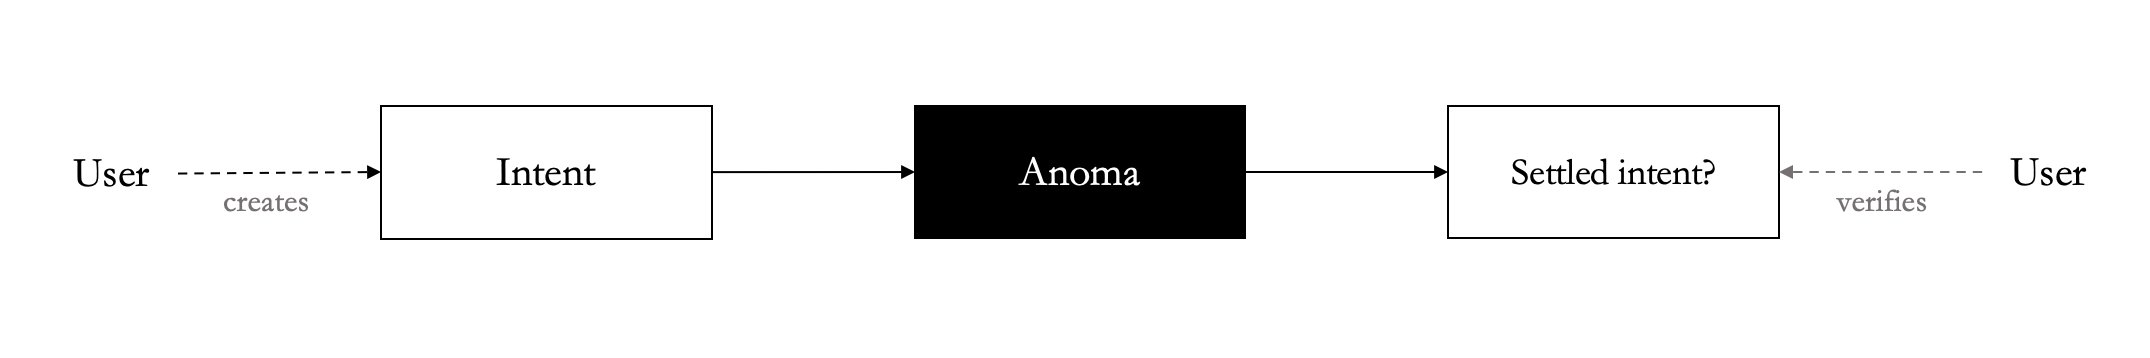
\includegraphics[width=0.9\textwidth,keepaspectratio]{figs/user-applications}
\caption{End-user interfaces of applications on Anoma}
\end{figure*}

\subsection{Fractal instance}\label{fractal-instance}

A \emph{fractal instance} is an instance of the Anoma consensus and
execution protocols operated by a set of networked validators. In
general, fractal instances are security domains, in that they are
operated by a particular set of validators, of which the user must trust
a quorum; concurrency domains, in that they maintain a full order of
only the transactions which they execute; and data availability domains,
in that external observers can query the fractal instance to retrieve
parts of its state. Fractal instances are sovereign, in that they do not
depend on any other part of the fractal instance graph for continued
correct execution, although their validator sets may overlap, a property
which can be exploited in certain cases to provide multi-chain atomic
settlement. Fractal instances, in order to be compatible with all
features of the network, must implement the Anoma consensus and
settlement protocols according to the specification, but they can vary
in their chosen sybil-resistance mechanisms, execution pricing, and
local governance of protocol versioning, economic distribution regime,
and irregular state transitions handling.

\section{Programming model}\label{programming-model}

Considering the architecture of Anoma from the perspective of users with
preferences over states of the system, one might ask the question: why
are there applications at all? Cannot users merely articulate their
preferences and the system enact them, without further component
intermediation? In principle, they can, but the search space of solvers
and difficulty of coordinating the relations between the state of the
ledger and state of the world would be computationally intractable
without coordination on particular forms of representation and
particular logics of preference expression and settlement. Applications
describe these particular forms, on which it is necessary to coordinate
in order to express, match, and settle intents, and in order to provide
simple and accurate interfaces for users.

\subsection{Application components}\label{application-components}

An application on the Anoma architecture consists of intent formats, an
application state validity predicate, user validity predicate
components, solver algorithms, and one or many user interfaces.

\begin{itemize}
\item
  \emph{Intent formats} describe the form and semantics of particular
  intents utilised by the application, which must be created by the user
  interfaces, understood by intent gossip nodes, matched by solvers, and
  validated by the application's validity predicates.
\item
  The \emph{application state validity predicate} encodes the relation
  governing valid state transitions of the application's
  state.
\item
  \emph{User validity predicate components} encode the relations which
  users can approve in order to allow for safe interactions with this
  application.
\item
  \emph{Solver algorithms} instruct a solver how to match this
  application's intents and form valid transactions.
\item
  Finally, \emph{user interfaces} present users with a graphical or
  textual view of and controller for the application in question.
\end{itemize}

\subsection{Application portability}\label{application-portability}

By default, applications are portable across fractal instances, and
application state validity predicates may also reason about security and
concurrency domains in order to allow for safe interaction between users
of an application across these domains.

Although nothing ties a particular interface to a particular
application, Anoma's intent gossip network is capable of
acting as a data availability layer for interface code, in a way which
allows secure synchronised interface and application versions.

\subsection{Application security model}\label{application-security-model}

In Anoma, users distrust applications. Applications are never granted
un-restricted access to modify a user's state. All state
entries carry an explicit owner, and the validity predicate associated
with that owner must authorise all changes to that state. Instead of
authorising à la \texttt{transferFrom}, users add components to their
validity predicates which allow for specific interactions with a
specific application, which can then be performed non-interactively from
the perspective of the user, if they have granted the application
license to do so. These components can be altered or revoked at any
time, and allow for "defence-in-depth", e.g. prevent transfers of more
than X within time bound \texttt{t}.

\subsection{Application state model}\label{application-state-model}

Anoma assumes clients are \emph{stateful} - they are treated as
components of the distributed system. Messages will only be sent once,
and can be marked as delivered, in which case they will not be kept
around. Message history can be reconstructed by reprocessing historical
transaction archives.

\section{Applications}\label{applications-secapplications}

The architecture of Anoma is suitable for any application desiring to
provide counterparty discovery, solving, and settlement for particular
forms of preferences over a particular semantic domain. Here we
enumerate several primitives that Anoma exposes to application
developers. We then list several examples of contemporary decentralised
applications and how they would benefit from Anoma's
architecture. Followed by the description of novel decentralised
applications which have hitherto been impractical or impossible to
develop due to the constraints of existing architectures.

\subsection{Novel primitives for
applications}\label{novel-primitives-for-applications}

Anoma exposes several new primitives to application developers:

\begin{itemize}

\item
  Incentivised data availability, for data which is expected to be used
  in the creation of future transactions, provided by the intent gossip
  layer (see \textbf{Section 6: Architectural instantiation}).
\item
  Programmable solvers, provided by intent gossip nodes running solver
  algorithms, to which can be outsourced the computational task of
  finding an atomic state transition (transaction) involving many
  parties which simultaneously satisfies all of their preferences.
\item
  Programmable threshold decryption, provided by Ferveo
 ~\cite{bebel2022ferveo}, which can be used to implement on-demand
  batching and enforce configurable fairness properties on the
  processing of application-specific state transitions submitted within
  a quantised period of logical time.
\item
  Programmable privacy, provided by ZKP systems and fully homomorphic
  encryption (FHE), which can be used to separate verification of
  properties of data from knowledge of the data itself. Application
  developers can leverage programmable privacy to build applications
  that handle transparent, shielded, and private state in the same
  application.
\end{itemize}

These primitives taken together provide the flexibility required to
build complex user-friendly applications which provide the desired
game-theoretic, privacy, and latency properties, such as decentralised
quadratic voting and quadratic funding, voting through incentivised data
availability, settlement through solvers, privacy \& receipt-freeness
through ZKPs and HE.

\subsection{Application examples}\label{application-examples}

\subsubsection{Contemporary decentralised
applications}\label{contemporary-decentralised-applications}

Here we list example of collections of contemporary applications that
follow the intent, counterparty discovery, and solving design pattern,
but that are at the moment application specific and rely on at least one
single-operator component.

\paragraph{Decentralised exchanges}\label{decentralised-exchanges}

Contemporary decentralised exchanges for both fungible and non-fungible
tokens, such as 0x, CoWSwap, Uniswap, Wyvern, and Seaport, require both
counterparty discovery, solving, and settlement, besides other
requirements such as batched/fair execution. At the moment, such
projects either use the blockchain itself for counterparty discovery
(Uniswap) or operate single-operator orderbooks controlled by specific
parties (0x, Wyvern, Seaport, CoWSwap), which tend to be trusted for
fair ordering and optimal execution. Using Anoma, these parties could be
replaced by the peer-to-peer intent gossip and distributed solving
layer, which generalises through arbitrary trades. Orders to buy or sell
particular assets would instead be broadcasted across the intent gossip
network as intents, matched by a solver, who could collect any number of
intents in order to balance a trade, and submitted for settlement to the
fractal instance holding the assets in question. Threshold decryption
can be used for fairness across batches.

\paragraph{Rollups}\label{rollups}

Existing rollup architectures, both optimistic ones such as Arbitrum,
Optimism; and zero-knowledge ones, such as ZkSync or StarkNet, operate
with a single-operator sequencer and solver responsible for ordering
transactions, calculating state updates, and submitting updated states
to the root chain, in these cases, Ethereum. This sequencer is trusted
with fair ordering and optimal solving, and can selectively omit
transactions, so some projects have expressed a desire to decentralise
the sequencer. As a decentralised sequencer is simply a consensus
instance, such rollups could instantiate an Anoma fractal instance,
using Typhon consensus, to operate their sequencer, and submit
zero-knowledge or optimistic proofs of execution to Ethereum as they
currently do.

\paragraph{Public goods funding}\label{public-goods-funding}

Quadratic funding (QF), as implemented by Gitcoin, requires both
counterparty discovery, solving (as the funding
provider's payouts depend on individual donations), and
settlement. Using Anoma, QF can be implemented in a manner which
preserves individual privacy and provides excellent UX (e.g., donating
to projects carries no fees). The funding provider, project creators,
and all individual donators each author intents reflecting their
willingness to commit funds, execute on a project, and donate,
respectively. A solver algorithm matches these intents and creates a
single transaction to settle at the end of the QF round, while the
funding provider can pay the settlement fees. Amounts of donations must
be public in order to perform the QF calculations, but individual
identities can be kept private using Anoma's private
execution environment. Expressive intents can also capture additional
dimensionality which is difficult to represent in a simpler QF model -
for example, many projects require a certain amount of funding in order
to do anything at all, and only wish to receive funding (and commit to
action) should a certain threshold be met. This can be expressed as a
constraint in the intent, and the solver must either find enough funding
to meet the threshold or omit the project, as desired, in order for the
final settlement transaction to be valid.

\subsubsection{Novel applications}\label{novel-applications}

Here we sketch some novel decentralised applications that can be built
using Anoma's architecture: DAOs 2.0, runtime rollups,
multiparty multivariate bartering, private auctions, and local episodic
games.

\paragraph{DAOs 2.0}\label{daos-20}

Decentralised autonomous organisations (DAOs) hold the twin promises of
organisational \emph{operational transparency}, in that the rules for
decision-making are articulated and executed in the same code, which
anyone can read, and \emph{operational verifiability}, in that any past
actions of the organisation can be proven to a third party to be
consistent with this rule set. In present instantiations, however, they
obtain transparency and verifiability by execution on a public
blockchain, which comes at the cost of privacy.

Operational privacy allows organisations to present, and prove with
verifiability, specific data about the organisations inputs and outputs
(e.g. quarterly funding disclosure for a non-profit) without revealing
every aspect of decision-making, which is a lot of data from which
someone can easily cherry-pick to misrepresent what's
really happening, or which members of the public with other agendas
(perhaps operating a competing organisation, or with a personal bone to
pick with a member of the one in question) can use to start
bike-shedding debates or otherwise interfere with organisational
operations.

Anoma's architecture allows for the creation of private
DAOs which need make no such compromise: they can keep both
decision-making rules and data private, visible only to parties within
the organisation, but prove arbitrary properties of each to the world as
they choose.

In particular, this system could be used to instantiate something like
the plural money system~\cite{pluralmoney}. Communities could themselves
create private DAOs, controlled by members of the community, with
internal community currencies, community-owned SALSA-allocated assets,
and limitations/taxes on wealth transfer outside the community.

\paragraph{Runtime rollups}\label{runtime-rollups}

Let us take a "rollup" to be the separation of computation and
verification such that the verification can be suitably replicated for
improved fault-tolerance while the computation need not be. In systems
which rely on imperative semantics, and where end-users are signing
particular imperative execution paths, rollups are long-lived and must
be specifically specified by users. In Anoma's
declarative architecture, since users sign intents expressing properties
which the execution is required to satisfy rather than any particular
execution path, rollups can be created at runtime depending on dynamic
demand, and markets for compute may be used rather than replication
where doing so is cheaper.

\paragraph{Multiparty, multivariate private
bartering}\label{multiparty-multivariate-private-bartering}

Consider three friends, Alice, Bob, and Charlie, a hotel operator David,
a festival producer Eve, and a train company Deutsche Bahn. The festival
runs for three weekends in July near Potsdam. Alice, Bob, and Charlie
wish to attend the festival together, on the same weekend, and take
trains from their respective home towns of Berlin, Zurich, and
Amsterdam. They're flexible about the particular
weekend, and would like the combined price of train tickets, hotel
rooms, and festival passes to be as low as possible. Eve wants to sell
tickets to his festival, which are fixed-price based on his costs plus
markup, but sometimes resold by parties who purchase them early on then
later realise that they cannot attend. Deutsche Bahn sells train tickets
with variable prices based on demand, David likewise for hotel rooms
(and she has both single rooms suitable to host one person and quadruple
rooms suitable to host four). Alice, Bob, and Charlie are happy to room
with another person, as long as they are also attending the festival
(they view this as good evidence of a likely friendship).

In the world today, Alice, Bob, and Charlie might go to the
festival's website to look for ticket availability, then
try to check hotel and train prices across the three possible weekends
and compile a spreadsheet in order to figure out what their costs might
be. Of course, while they're busy compiling the
spreadsheet, someone else looking to travel could book their hotel room
or train seat, and they'd be out of luck. Worse, they
could book a hotel room for a particular weekend, then find out that the
train tickets are unavailable and be unable to change the hotel room (at
least without paying a cancellation fee).

Alice, Bob, Charlie, David, Eve, and Deutsche Bahn could all use Anoma
as a substrate for multiparty private bartering. Each party would author
an intent with their preferences, and all intents would either be
matched atomically (meaning that train tickets, hotel rooms, and
festival passes are booked for all of Alice, Bob, and Charlie in
correspondence at once) or not at all. Using private bartering,
\emph{what} all parties want is public, but \emph{who} they are need not
be revealed.

This can also be used for simpler cases, such as fungible tokens. Users
can author intents capturing the semantics of market \& limit orders,
and also more complex algorithms such as an AMM. Expressed in intent
form, an AMM order is simply a price curve along which one is willing to
swap two assets (\texttt{xy\ =\ k}). Users can author AMM intents for
the full price range or any subrange (similar to Uniswap v3). Unlike
on-chain AMMs, this does not require sending transactions or locking any
assets up.

\paragraph{Private auctions}\label{private-auctions}

Independent of more long-term reasons, auctions often benefit from
privacy for game-theoretic reasons: a sealed-bid second-price auction
gives bidders reason to bid their true value, but requires bid privacy
in order to work. Using Anoma, such auctions could be conducted
privately, in two different ways. The first and most immediately
feasible way is to use programmable threshold decryption to keep all
bids encrypted until the auction deadline has passed, then decrypt them
all at once, select the highest bidder as the winner and charge them the
second-highest price. This can be combined with other privacy techniques
for concealment of identity. FHE can also be used to implement private
auctions, by performing the bid selection directly as operations on the
bids submitted as ciphertexts.

\paragraph{Local episodic private
games}\label{local-episodic-private-games}

Consider a digital re-enactment of a game of poker. Games of poker are
episodic, in that (even if bets are being placed and winners reported to
a leaderboard) no interaction or ordering takes place between different
games - if users are submitting actions, actions taken by users within
the same game must be ordered with respect to actions taken by other
users in that game, but not with respect to actions taken by any others.
Anoma's fractal instance architecture can instantiate
this structure efficiently: players, when they start a poker game,
launch a temporary consensus instance (simply operated between
themselves) to order state transitions within that game, then submit the
results at the end to a poker tracking/statistics application on a more
long-running fractal instance. This fractal instance can be run on LAN
for low-latency, and transactions need not have any cost (since the set
of who can submit them is restricted to the players).

Poker also requires privacy, primarily keeping a private hand and
periodically revealing cards, and randomness (for the deck shuffle),
which can be provided by the private execution system and threshold
signatures from the threshold cryptosystem in Anoma, respectively.

\section{Architectural instantiation}\label{architectural-instantiation}

The Anoma architecture requires many individually intricate
subcomponents which can be instantiated in a variety of ways with
different performance, complexity, and ergonomic trade-offs. Here we
sketch the abstract interfaces required of necessary subcomponents and
summarise our current development directions in instantiating them.

\subsection{Gossip}\label{gossip}

The Anoma gossip system is a pseudonymously identified,
path-authenticated, fault-accountable sparse overlay network. In
contrast to conventional peer-to-peer gossip networks, this system is
designed to operate privately by default, with optional attestations.
Nodes are identified by cryptographic keys and all messages are
encrypted to their recipient and signed by their sender. Nodes craft \&
enforce local rules around message validity, rebroadcast, and retention.
Combined with a settlement ledger and path-authentication-based fees,
this provides an incentivised data availability layer for
transaction-relevant data, which is used within the Anoma architecture
by users to broadcast intents, which are sent around until solvers find
counterparties, create transactions, and submit them to fractal
instances for settlement. Nodes maintain a local trust graph and ruleset
around message content validity and rebroadcast criteria. The Anoma
gossip system uses an explicit trust model, where the underlying
physical network is distrusted, new nodes bootstrap with a set of
trusted peer public keys, and nodes maintain trust relations over time,
keeping track of who introduced them to whom and applying changes in
trust recursively along the trust graph.

\subsubsection{Node model}\label{node-model}

Nodes in the gossip network are assumed to possess a private key, the
corresponding public key to which is used as identification. Nodes must
totally order and sign all messages which they send, which are unique.
Signing two messages with the same nonce is an accountable fault.

In traditional P2P gossip systems, nodes are primarily identified by
their IP address, which refers to a physical network destination and is
assumed to be long-lived. By contrast, in the Anoma gossip system, nodes
are primarily identified by their public key, which can list and
periodically rotate IP addresses at which it could potentially be
reached (but which a sender does not necessarily need to know in order
to send messages). This can be seen as a sort of virtual gossip network,
with identity persistence based on secret information (the private keys)
which can be freely moved across physical substrates. Local caches of
physical routing latency are kept in order to maintain a relatively
efficient mapping of the spatially non-local virtualised network into
the spatially local physical one.

This choice of structure also allows for a conceptually elegant
virtualisation of fault-tolerant subsystems: a threshold cryptosystem in
combination with consensus (in order to provide ordering) effectively
virtualises many nodes as one node, with the threshold key used for
incoming and outgoing messages and shares for threshold decryption and
threshold signing internally rebroadcast around for reconstruction
(encrypted to individual node public keys for privacy). In contrast to
other blockchain systems, Anoma's gossip network is not
sharded on the basis of security domains (compare to independent
blockchain mempools), but rather simply sparse, where real-time demand
can inform connection choices and routing tables.

\subsubsection{Path authentication}\label{path-authentication}

Anoma's gossip system provides \emph{path
authentication}: the receiver of a message can verify a chain of
signatures recursively back all the way to the original sender, such
that each party in the message chain can be verified to have authorised
the next send, and can be both potentially paid for participating in
gossip and held accountable for inconsistent ordering across messages.
This is accomplished simply by keeping an ordered list of signatures in
the message header, which can all be checked by the recipient for
correctness and linkage consistency. For efficiency and privacy,
validity checks may be compressed and inner path identities may be
hidden using ZKPs, which the recipient then verifies as a part of
receiving the message.

\subsubsection{Gossip incentives}\label{gossip-incentives}

The path authentication system described above can be used to provide a
form of gossip incentive whereby a user can broadcast an intent and
offer payment to any nodes who participate in a chain of gossip which
leads to its eventual settlement. The user simply includes a small fee
(the semantics of which are chosen at runtime) which they allow gossip
nodes to malleate, so that each node, when forwarding the message, can
choose to take a portion of the fee for themselves. If the node can
settle the intent by combining it with others, crafting a valid
transaction, and submitting it to the appropriate fractal instance, they
can claim the fee immediately. If not, the node can choose how much fee
to take for themselves before they forward the message. Of course, they
can take all the fee, but then there would be no reason for other nodes
to rebroadcast or settle the intent, so the node would receive nothing.
Nodes can thus be expected to rebroadcast intents taking only enough of
the fee such that the expected benefits of potential settlement outweigh
the opportunity cost of potentially being able to settle it themselves
(but the user can broadcast their intent to many parties, so an
individual node who cannot immediately settle it is unlikely to be the
first to be able to).

\subsection{Consensus}\label{consensus-1}

The consensus component is an algorithm by which many nodes can be
abstracted as one virtual node, which will be correct subject to certain
assumptions about the correctness of the constituent nodes (generally
$\frac{2}{3}$). Just as individual
nodes operate a deterministic state machine and send and receive
messages in a local total order, virtual nodes created by use of the
consensus algorithm operate a deterministic (replicated) state machine
and send/receive messages in a total order. The consensus algorithm is
responsible for abstracting many nodes into this virtual node by
gossiping, ordering, and executing transactions (incoming messages),
then finalising the updated states (outgoing messages) in a verifiable
manner.

At present, the consensus component in Anoma is instantiated by
Typhon~\cite{typhon}, which draws substantially from Heterogeneous
Paxos~\cite{sheff2021heterogeneous}, Narwhal~\cite{danezis2022narwhal},
and Tendermint~\cite{buchman2018latest}.

\subsubsection{Ordering}\label{ordering}

The ordering component of consensus is responsible for ordering
transactions prior to execution, where nodes participating in consensus
must agree on the ordering and ensure that all transactions so ordered
are available to them for execution.

\subsubsection{Execution}\label{execution-1}

The execution component of consensus is responsible for executing
transactions on which an order has already been agreed, updating the
state to reflect the results of transaction execution, and finalising
the updated state so that external parties can inexpensively verify
properties of it.

\subsection{Execution environments}\label{execution-environments}

The execution environment of Anoma is a runtime responsible for
partitioning and permissioning state and code to allow for safe
interoperation of mutually distrusting programs, abstracting
transparent, shielded, and private state changes and providing
appropriate primitives for cryptographic operations, and handling
cross-fractal instance state verification as well as synchronous and
asynchronous cross-fractal-instance messaging. These three
responsibilities of abstraction are orthogonalised into three
components: the validity predicate subsystem, the unified
transparent/shielded/private execution environment (Taiga), and the
transparent execution environment (Typhon EE).

\subsubsection{Validity predicate
subsystem}\label{validity-predicate-subsystem}

The validity predicate (VP) subsystem is responsible for partitioning
and permissioning state and code in order to allow for safe
interoperation of mutually distrusting programs. This is accomplished by
splitting the keyspace of transparent, shielded, and private state into
mutually exclusive prefix spaces, where the first part of a key
corresponds to ownership by a specific validity predicate, stored at a
sentinel key within that prefix. Whenever state within a particular
prefix is altered, the validity predicates associated with that prefix
are called, and they can choose to accept or reject the transaction.
Validity predicates can also choose to require that other validity
predicates also accept.

The validity predicate subsystem is itself implemented as a validity
predicate and can in principle be instantiated recursively. The
subsystem is also responsible for enforcing limitations on what data is
accessible to VPs.

\subsubsection{Taiga Unified EE}\label{taiga-unified-ee}

The Taiga unified execution environment is responsible for handling
transparent, shielded, and private data access and operations.

\paragraph{Data privacy domains}\label{data-privacy-domains}

Transparent data is represented as a mutable key-value tree, where keys
can be read, written, and deleted, and prefixes can be iterated over.

Shielded data is represented as an immutable append-only note set, where
each note can be either consumed once or many times. Each note includes
a key, value, and owner key, to which an encryption of the note contents
must be available.

Private data is represented as a mutable key $\to$ ciphertext
mapping, where keys can be read, written, and deleted, and ciphertexts
can be operated on using special homomorphic instructions.

\paragraph{Cross-domain transit}\label{cross-domain-transit}

Conversion between the three data realms is handled as follows:

\begin{itemize}

\item
  Transparent $\to$ Shielded: Transparent data can be read or
  computed over in the course of execution, and then written into a
  shielded note.
\item
  Transparent $\to$ Private: Transparent data can be read or
  computed over in the course of execution, and then encrypted to the
  threshold key.
\item
  Shielded $\to$ Private: Shielded data can be computed over
  in zero-knowledge, and then encrypted to the threshold key, where
  correct encryption is proved in zero-knowledge and only the encrypted
  value is revealed to the operator.
\item
  Shielded $\to$ Transparent: Properties of shielded data can
  be proved in zero-knowledge and then revealed to the operator along
  with the proof.
\item
  Private $\to$ Transparent: Private ciphertexts can be
  decrypted using threshold decryption. This process is asynchronous.
\item
  Private $\to$ Shielded: Private ciphertexts can be
  re-encrypted to another public key and thus become shielded data. This
  process is asynchronous.
\end{itemize}

\subsubsection{Typhon Transparent EE}\label{typhon-transparent-ee}

The Typhon execution environment is the lowest-level execution
environment, designed to impose only the minimal requirements and
structure required by Typhon for transaction ordering and concurrent
execution.

The Typhon execution environment has only transparent state, which is
organised in a key-value tree. Transactions declare parents of all
subtrees of keyspace within which they will read and write. Using this
information, Typhon can identify transactions which touch only
non-overlapping regions of state and thus order transactions for
concurrent execution. This execution environment does not itself have
any state semantics for private data or state/code partitioning. Further
structure is specified by a root validity predicate, stored at a
particular sentinel key, which is called as a part of all transactions.

The Typhon EE is also responsible for handling asynchronous message
passing across fractal instances and synchronous (atomic) message
passing within chimera chains. The EE handles transport, ordering, and
verification, while message semantics are left to higher execution
abstraction layers.

\subsection{Compilation stack}\label{compilation-stack}

In order to provide a unified black-box application development
interface, the Anoma implementation includes a new language, Juvix, and
a compiler stack, designed in tandem to allow developers to write
formally verified, privacy-preserving, fault-tolerant distributed
applications.

A great deal of research work into the compiler stack remains and this
section should be considered a work in progress. Several components
described herein are only partially implemented and alternatives are
still under active consideration.

\subsubsection{Juvix}\label{juvix}

Juvix is a high-level function language which compiles to a variant of
the simply typed lambda calculus. Programs written in Juvix can express
and reason about public, shielded, and private data and operations.
Juvix's lambda calculus output language can be compiled
to RISCV or WASM through C, or can be compiled to the abstract
categorical operations of the AVM which can in turn be instantiated as
polynomials, the input language of VampIR.

\subsubsection{AnomaVM}\label{anomavm}

The AnomaVM (AVM) is a distributed abstract categorical virtual machine.
The AVM is designed to capture information theoretic semantics of
multiparty interactions and compute without fixing concrete
cryptographic representations/instantiations or operational execution
semantics. An AVM program directly references agents by role, who can
reason about each others state transitions and states through proofs of
execution and authentication, and who can send and receive messages to
and from each other.

An AVM program itself specifies agents only abstractly, but it can be
executed (or compiled, then executed) by any agent, who must specify the
role they wish to play (this is a sort of local naming system). The AVM
can be compiled through LLVM for transparent execution, and through
VampIR for circuits suited to ZKP or FHE execution.

As an operationally neutral abstract representation, the AVM is also the
level at which the Anoma architecture defines cost semantics and
identity of programs, e.g. different parties may compile AVM programs to
different concrete cryptographic and transparent backends for execution.

\subsubsection{VampIR}\label{vampir}

VampIR is a language and compiler designed to provide an abstract
representation of polynomials, circuits, and constraint systems which
can be compiled to different concrete proof systems. The IR is designed
to capture the denotational semantics of circuits while remaining
agnostic to operational semantics of instantiation in various proof
systems and cryptographic backends, including ZKP and FHE.

\subsection{Fractal instance
components}\label{fractal-instance-components}

\subsubsection{Sybil resistance}\label{sybil-resistance}

Fractal instances must provide a Sybil resistant mechanism in order to
assign voting power in consensus. This can be proof-of-stake,
proof-of-authority, hybrid (partially fungible) proof-of-stake, or some
form of liquid democracy based on the cryptographic identity substrate.

\subsubsection{Governance}\label{governance}

Fractal instances may provide a governance mechanism for enacting
irregular state changes by a (somewhat) more regular process than what
would take place without any such system. This governance mechanism
itself requires Sybil resistance, which can be the same as used in
consensus or a slight variant.

\subsubsection{Resource pricing}\label{resource-pricing}

Fractal instances must provide a Sybil resistance mechanism for
performing expensive computational operations upon the receipt of
messages which can be sent by anyone in an open network. This Sybil
resistance mechanism could be based on fees paid in a network token,
identity-based quotas or subscriptions of compute, storage, etc., or low
flat per-message limits in combination with network-based rate limiting.

\section{Future directions}\label{future-directions}

\subsection{Private counterparty
discovery}\label{private-counterparty-discovery}

The trade-off axis between counterparty discovery, fairness, and privacy
is quite fundamental: in order to find a counterparty in any way more
efficient than random testing, you must provide some information about
your preferences, which entails a corresponding loss of privacy, and in
order to provide fairness across a larger set of parties in cases of
uncertain information (e.g. variable prices), you must make your
preferences public to a larger set of solvers who can see more intents
at once and compete to find the fairest solutions.

Encrypted solving (solving intents which are completely private to the
solver), while possible in principle, pairs the already NP problem of
solving with the overhead of heavy-duty HE, and is likely to remain
infeasible in the near future, but research into improved algorithms,
application-specific solutions, and dedicated hardware could bring these
overhead costs down over time.

\subsection{End-to-end behavioural
verification}\label{end-to-end-behavioural-verification}

Anoma's architecture covers the domain from (abstract)
Turing machines operating node software to (abstract) users authoring
intents, and provides guarantees for the behaviours of the system with
respect to the latter given certain assumptions about the behaviours of
the former. In practice, safe usage of a deployment of Anoma depends not
only on the correctness of this system but also on the correctness of
the hardware utilised by nodes and the correctness of interfaces
utilised by users. Eventually, this verification could be extended
further into the interface and hardware domains.

\section{Acknowledgements}\label{acknowledgements}

\nocite{*}
\bibliography{ref.bib}

% \appendix
% \section{Some extra stuff}


\end{document}
